
\documentclass[11pt]{article}
\usepackage[margin=1in]{geometry}
\usepackage{caption} %For captioning objects
\usepackage{subcaption} %sub-captioning pictures
\usepackage{graphicx} %to include graphics
\usepackage{hyperref} %for clickable references
\usepackage{listings} %to write code listings
\lstset{language=R, breaklines=true}  
\usepackage[mathcal]{euscript} %for curly S
\usepackage{mathtools}
\usepackage{float} %so figures can be placed "here"

%Defining commands for math symbols
\usepackage{amsmath} %to enable split equations
\usepackage{statmath} %for plim. Be careful, it has already \E and \V.
\usepackage{amssymb} %to enable mathbb
\newcommand{\R}{\mathtt{R}} %Software R
\renewcommand{\E}{\mathbb{E}} %expectation
\usepackage{bbm}
\newcommand{\1}{\mathbbm{1}}
\renewcommand{\V}{\mathbb{V}} %variance
\newcommand{\N}{\mathcal{N}} %normal distribution
\newcommand{\U}{\mathcal{U}} %normal distribution
\renewcommand{\P}{\mathbb{P}} %proba, renewcom since \P already exists
%Regression variables in vector form
\newcommand{\y}{\boldsymbol{y}} 
\newcommand{\x}{\boldsymbol{x}} 
\newcommand{\z}{\boldsymbol{z}} 
\newcommand{\yhat}{\boldsymbol{\hat{y}}} 
\renewcommand{\u}{\boldsymbol{u}} 
\newcommand{\uhat}{\boldsymbol{\hat{u}}}  
\newcommand{\Px}{\boldsymbol{P}}  
\newcommand{\Mx}{\boldsymbol{M}}  
\newcommand{\A}{\boldsymbol{A}}  
\newcommand{\X}{\boldsymbol{X}}  
\newcommand{\Z}{\boldsymbol{Z}}  
\newcommand{\e}{\boldsymbol{e}}  
\renewcommand{\r}{\tilde{r}}  
%\renewcommand{\r}{\boldsymbol{r}} 
\renewcommand{\i}{\boldsymbol{\imath}} 
\newcommand{\alphab}{\boldsymbol{\alpha}}  
\newcommand{\betab}{\boldsymbol{\beta}}  
%opening

\newcounter{daggerfootnote}
\newcommand*{\daggerfootnote}[1]{%
	\setcounter{daggerfootnote}{\value{footnote}}%
	\renewcommand*{\thefootnote}{\fnsymbol{footnote}}%
	\footnote[2]{#1}%
	\setcounter{footnote}{\value{daggerfootnote}}%
	\renewcommand*{\thefootnote}{\arabic{footnote}}%
}


\title{Problem Set 6 - ECON 880\\
	\small Spring 2022 - University of Kansas}
\author{Gunawan, Minh Cao}


\begin{document}

\maketitle	
\section*{Question 1}






\begin{tabular}{ |p{3cm}||p{3cm}|p{3cm}|p{3cm}|  }
 \hline
 \multicolumn{4}{|c|}{Question 1} \\
 \hline
               & $n=3$ &$n=5$&$n=11$\\
 \hline
    Trapezoid      & 0.081359     &0.041771 &   0.01481\\
     Gauss-Chebyshev   &     0.036964    & 0.012382     &0.0024208\\
 Gauss-Legendre   &0.0051406   & 0.0015098 & 0.00020904\\
  \hline
\end{tabular}
\begin{itemize}
\item True value of the integral = 34.920804 
\end{itemize}

\section*{Question 2}
\begin{itemize}
\item True value of the integral = 34.920804 
\item It is clear that the  pseudo-random error does not converge to zero, however it is bounded by 0.08. The ) uniformly spaced grid method converges to zero, however if the number of nodes are less than 3000, the   pseudo-random method does better the uniformly spaced grid since the lower bound of the uniformly spaced grid method is 0.1.
\end{itemize}


\begin{figure}[h]
	\centering
		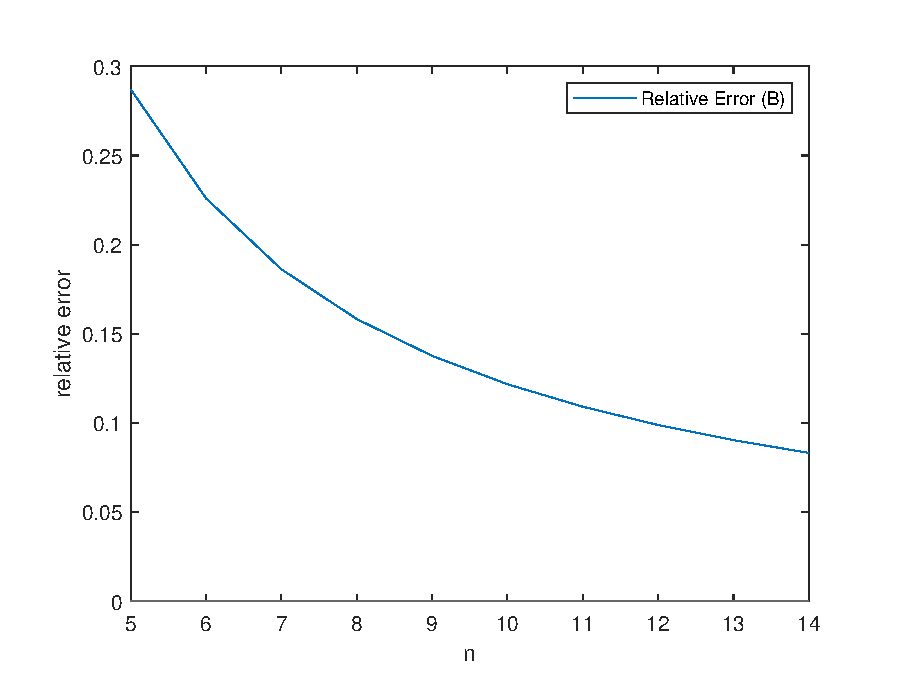
\includegraphics[width=\textwidth]{fig2.eps}
	\caption{ Pseudo-random error}
	\label{2a:1}
\end{figure}
\begin{figure}[h]
	\centering
		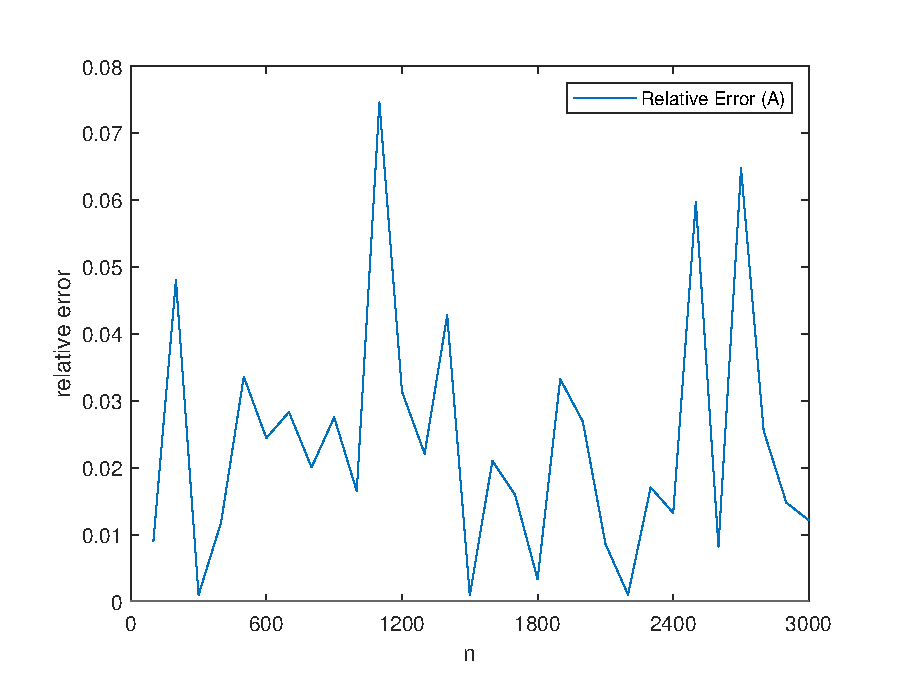
\includegraphics[width=\textwidth]{fig1.eps}
	\caption{Uniformly spaced grid error}
	\label{2a:1}
\end{figure}

\end{document}

